\section{Introduction}\label{sec:introduction}
ARC-AGI-3 asks an agent to discover the rules and objectives of unfamiliar interactive games and scores it by how efficiently it acts compared with a human baseline \citep{arc2026technical}. The agent studied here used Claude Opus 5.5 as its language model. Its harness gathered relevant evidence from the game, managed memory, and executed the model's chosen actions. The harness determined what information was available to the model. In the baseline, this included the current game board, up to two earlier board positions, the eight most recent actions, and up to eight hypotheses about the game rules and objectives that the model wrote.

In level 2 of the baseline run of \texttt{bp35}, an ARC-AGI-3 game, the model's piece rose into a purple tile at action 23 and the game ended. The model then recorded that rising into tiles of that kind was fatal. By action 32, this fatal move was no longer among the eight most recent actions shown to the model. At action 33, the model marked the rule as tentative, meaning it treated the rule as uncertain. By action 36, the model's notes no longer contained the rule. Later, the model described the same purple tiles as ``hazards or goals'' with an unknown role. At action 48, the piece rose into another purple tile and the game ended again (Figure~\ref{fig:bp35-example}) \citep{dai2026memoryfix}.

\begin{figure}[htbp]
\centering
\begin{tabular}{@{}c@{\hspace{8pt}}c@{\hspace{8pt}}c@{\hspace{8pt}}c@{}}
\board[0.235\linewidth]{baseline-forgetting-a.png} & \board[0.235\linewidth]{baseline-forgetting-b.png} &
\board[0.235\linewidth]{baseline-forgetting-c.png} & \board[0.235\linewidth]{baseline-forgetting-d.png}\\[1pt]
\footnotesize (a) Before action 23, click ringed & \footnotesize (b) Action 23, frame 15 of 28 &
\footnotesize (c) Before action 48 & \footnotesize (d) Action 48, frame 17 of 32
\end{tabular}\\[7pt]
{\footnotesize
\begin{tabularx}{\linewidth}{@{}rlY@{}}\toprule
Action & Status & The model's note about the purple tiles, in the reply that chose the action\\\midrule
25 & Supported & ``The f objects with b0b at the bottom are hazards: rising into them causes GAME\_OVER. [\ldots]''\\
33 & Tentative & ``The f/b0b objects are hazards, and they sit above every column from x37 to x53. [\ldots]''\\
36 & & No note about the tiles, in this reply or the next five\\
42 & Tentative & ``The f tiles with b0b bottoms are hazards or goals. Their role is unknown, so avoid them for now.''\\
48 & Tentative & ``The f tiles with b0b bottoms are hazards or goals; their role is unknown.''\\
50 & Supported & ``The f tiles with b0b bottoms are downward spikes. If the piece rises to directly beneath one, it dies and the game ends. [\ldots]''\\\bottomrule
\end{tabularx}}\caption{\textbf{The baseline repeated a fatal interaction after removing a learned hazard rule from its notes.} These observations come from \texttt{bp35}, level 2, with all four memory layers disabled. The piece is the small blue and yellow marker. The hazards are purple tiles with a yellow--white--yellow underside. In the notes, \texttt{f} denotes purple and \texttt{b0b} denotes the underside pattern. (a, b) At action 23, the model clicked the circled green tile above the piece, removing it. The piece rose beneath a purple tile, and the game ended. (c, d) At action 48, the model moved the piece one step left. It rose beneath another purple tile, and the game ended again. Panels (b) and (d) show intermediate animation frames for the reader. The model received only the final frame of each action, encoded as text. The table reproduces the model's notes and its own status labels from replies selecting the listed actions. Ellipses mark omissions. By action 32, action 23 had left the eight-action history shown to the model \citep{dai2026memoryfix}.}\label{fig:bp35-example}
\end{figure}


To see whether evidence from an earlier mistake would help the agent avoid repeating it, I returned to the saved model input just before action 48. I generated eight replies using the original input and eight using the same input with two earlier boards added. These boards showed the game immediately before and after the fatal move at action 23. All eight replies to the original input chose the fatal move. With the earlier boards added, four of eight replies chose it \citep{dai2026positiontest}.

The board test restored the earlier boards, while the evaluated harness kept a written lesson and asked the model to check its proposed action against that lesson. In the same test, five of eight replies given the model-written lesson and this check chose the fatal move, compared with all eight replies to the original input \citep{dai2026memoryfix}. These small tests examined the next decision at one saved position; they did not show whether the agent later completed the level.

I hypothesized that an agent with the model's lessons, rules, and notes about the board available at every decision would complete more levels and reach a higher Relative Human Action Efficiency (RHAE) than the baseline under the same action caps. The main study tested this hypothesis. The layered harness added four memory layers to the baseline. The model wrote lessons after a game over or an action that had no effect. An object ledger grouped board regions by appearance and kept the model's notes about them. A separate list preserved rules the model recorded during play. A level brief summarized how the previous level ended and what to investigate next.

All four layers used only the agent's own actions and observations. The model received no game-specific hints, could not use tools or access the game's source code, and had no memory from other games.

The difference showed in most games, not only in the average. The layered run scored higher than the baseline run in 20 of the 25 games, the same in four, and lower in one (Figure~\ref{fig:per-game-scores}).

\begin{figure}[htbp]
\centering
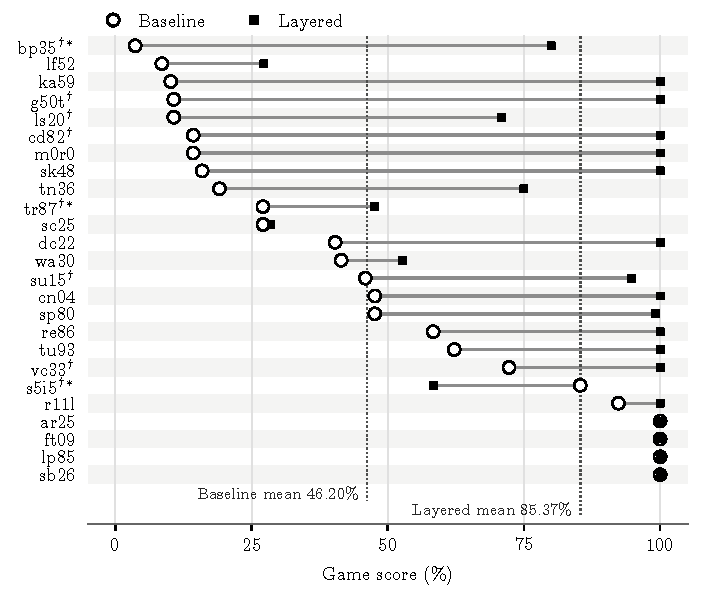
\includegraphics[width=0.66\linewidth]{figures/per_game_scores.pdf}
\caption{\textbf{The layered run scored higher than the baseline run in 20 of 25 games, the same in four, and lower in one.} Each row compares one baseline run and one layered run on the same game, under the same action cap. The rows run from the lowest baseline score to the highest. Open circles show the baseline score, filled squares show the layered score, and a line connects the two. The dotted lines mark the two mean scores. A dagger marks games used or studied during development. An asterisk marks layered runs stopped by repeated timeouts; the figure reports their scores at the point they stopped. The connecting lines show differences between two recorded runs; they do not show statistical uncertainty. Figure~\ref{fig:per-game-outcomes} adds levels completed and actions used.}\label{fig:per-game-scores}
\end{figure}


\Needspace{6\baselineskip}
This paper makes three contributions.
\begin{itemize}
\item \textbf{A layered harness} (Section~\ref{sec:layers}). I added four memory layers to the baseline harness, which had none of them. Figures~\ref{fig:lesson-game-over}--\ref{fig:level-brief} illustrate the layers with examples from the evaluated runs.
\item \textbf{A whole-game comparison on all 25 public games} (Sections~\ref{sec:result-score}--\ref{sec:result-budget}). I ran each harness once per game under the same per-game action caps. The layered harness scored 85.37\% RHAE, compared with 46.20\% for the baseline, completed 166 of 183 levels, compared with 125, and used 35.5\% fewer actions. Replaying the recorded actions through the ARC service confirmed both scores.
\item \textbf{Controlled tests of the level-brief package} (Section~\ref{sec:result-brief}). This package holds the level brief, the rule list, and two supporting features. Under a decision rule fixed before testing, it completed more levels in both test sets and met the benefit criterion in the second.
\end{itemize}

The thesis of this paper is that a language-model agent acts more efficiently on ARC-AGI-3 when its harness keeps the model's own lessons, rules, and notes about the board available at every decision. On these public games, the harness with all four layers performed better than the baseline. Because the whole-game comparison enabled all four layers together, it cannot determine how much each layer contributed. I used or studied eight of the tested games during development, and baseline summaries from all 25 informed it, so the results do not establish performance on unseen games. Section~\ref{sec:discussion} discusses these limits and the replication needed to address them. Appendix~\ref{app:analysis} presents the earlier 100-action baseline analysis and a two-game study of another system as context.
